The investigation of laser-matter interaction also involves exploring of specific themes of the ultra-relativistic regime, which requires extremely high intensities of the external field. These intensities, that are experimentally inaccessible at present, could be potentially achieved by tight-focusing and that would allow a broad spectrum of many multidisciplinary applications.

As mentioned in the previous chapter, various aspects of electromagnetic interaction are usually studied using sophisticated numerical simulation codes. Vast majority of these codes, however, use a paraxial approximation to prescribe the laser fields at the boundaries, and afterwards, the FDTD solver guides the beam across the simulation domain. The paraxial approximation is valid only if the angular spectrum of laser pulse is sufficiently narrow, therefore it is not possible to simulate tightly focused laser beams using this approach. As might be seen later, paraxial approximation in this case leads to a distorted field profiles which have strong impact on the results of laser-matter interaction.

Several interesting solutions, how to simulate strongly focused beams, have been already proposed [source]. Within this work, a simple and efficient algorithm for a Maxwell consistent calculation of the electromagnetic fields at the boundaries of the computational domain (also called laser boundary conditions) has been used and implemented into the PIC code EPOCH. Note, that this algorithm is able to describe laser beams with arbitrary shape.

\section{Calculation}



\section{Algorithm}

In the following section, the practical implementation of a boundary conditions based on the previously derived solution of Maxwell equations is presented. Assume, that the laser beam propagates in a forward direction along the axis z. In the beginning, it is necessary to prescribe the electric laser field $ \vec{E}_{0, \bot} (\vec{r}_{\bot}, t) $ in the plane $ \mathcal{P} $ at $ z = z_0 $. Note, that it can be defined by arbitrary function of space and time. The goal is then to find the fields $ \vec{E}_{\mathrm{B}} (\vec{r}_{\bot}, t) $ and $ \vec{B}_{\mathrm{B}} (\vec{r}_{\bot}, t) $ at the corresponding boundary $ z = z_\mathrm{B} $.

Consider that the transverse part of simulation domain is made of equidistant rectangular grid described by $ x^{i} $, $ y^{j} $, where $ i, j \in \left\lbrace 1, \ldots, N_{x, y} \right\rbrace $, and the grid steps $ \delta x $, $\delta y $. The simulation time $ t^{n} $, where $ n \in \left\lbrace 1, \ldots, N_{t} \right\rbrace $, is also divided into equidistant time steps of size $ \delta t $.

The algorithm allows to calculate fields $ \vec{E}_{\mathrm{B}}^{ij} (t) $ and $ \vec{B}_{\mathrm{B}}^{ij} (t) $ for any given time $ t $ from the interval $ \left[ t^{1} - \frac{z_\mathrm{B} - z_0}{c}, t^{N_t} - \frac{z_\mathrm{B} - z_0}{c} \right] $. In order to preserve clarity, the algorithm below is given in the exact form as in the original paper [source].

\begin{enumerate}
	\item Calculate $ \hat{\vec{E}}_{0, \bot}^{ijn} $ via discrete Fourier transforms in time:
	\begin{equation}
	\omega^n = \frac{2 \pi}{N_t \delta t} \left( -\frac{N_t}{2} + n \right),
	\end{equation}
	\begin{equation}
	\hat{\vec{E}}_{0, \bot}^{ijn} = \frac{\delta t}{2 \pi} \sum_{l=1}^{N_t} \vec{E}_{0, \bot}^{ijl} \e^{\i \omega^n t^l}, \quad n \in \left\lbrace 1, \dots, N_t \right\rbrace.
	\end{equation}
	\item Calculate $ \bar{\vec{E}}_{0, \bot}^{ijn} $ via two-dimensional discrete Fourier transforms in transverse space:
	\begin{equation}
	k_x^i = \frac{2 \pi}{N_x \delta x} \left( - \frac{N_x}{2} + i\right), \quad k_y^j = \frac{2 \pi}{N_y \delta y} \left( - \frac{N_y}{2} + j\right),
	\end{equation}
	\begin{equation}
	\bar{\vec{E}}_{0, \bot}^{ijn} = \frac{\delta x \delta y}{(2 \pi)^2} \sum_{l, m = 1}^{N_x, N_y} \hat{\vec{E}}_{0, \bot}^{lmn} \e^{- \i \: \left(k_x^i x^l + k_y^j y^m \right)}, \quad i, j \in \left\lbrace 1, \dots, N_{x, y} \right\rbrace.
	\end{equation}
	\item Calculate transverse electric field components at the boundary $ z = z_\mathrm{B} $:
	\begin{equation}
	k_z^{ijn} = \Re \sqrt{\frac{(\omega^n)^2}{c^2} - (k_x^i)^2 - (k_y^j)^2},
	\end{equation}
	\begin{equation}
	\bar{\vec{E}}_{\mathrm{B}, \bot}^{ijn} =
	\begin{cases} \bar{\vec{E}}_{0, \bot}^{ijn} \e^{\i k_z^{ijn}(z_\mathrm{B} - z_0)} & \text{for} \ k_z^{ijn} > 0 \\ 0 & \text{for} \ k_z^{ijn} = 0 \end{cases}.
	\end{equation}
	Symbol $ \Re $ stands for the real part of a complex number.
	\item Calculate longitudinal electric field components at the boundary $ z = z_\mathrm{B} $:
	\begin{equation}
	\bar{E}_{\mathrm{B}, z}^{ijn} = \begin{cases} -\frac{k_x^i \bar{E}_{\mathrm{B}, x}^{ijn} + k_y^j \bar{E}_{\mathrm{B}, y}^{ijn}}{k_z^{ijn}} & \text{for} \ k_z^{ijn} > 0 \\ 0 & \text{for} \ k_z^{ijn} = 0 \end{cases}.
	\end{equation}
	\item Calculate the magnetic field at the boundary $ z = z_\mathrm{B} $:
	\begingroup
	\renewcommand*{\arraystretch}{1.7}
	\begin{equation}
	\mathbb{R}^{ijn} =  \begin{pmatrix}
	-k_x^i k_y^j & (k_x^i)^2 - (\omega^n)^2/c^2 \\
	(\omega^n)^2/c^2 - (k_y^j)^2 & k_x^i k_y^j \\
	-k_y^j k_z^{ijn} & k_x^i k_z^{ijn} 
	\end{pmatrix},
	\end{equation} 
	\endgroup
	\begin{equation}
	\bar{\vec{B}}_{\mathrm{B}}^{ijn} = \begin{cases} (\omega^n k_z^{ijn})^{-1} \mathbb{R}^{ijn} \bar{\vec{E}}_{\mathrm{B}, \bot}^{ijn} & \text{for} \ k_z^{ijn} > 0 \\ 0 & \text{for} \ k_z^{ijn} = 0 \end{cases}.
	\end{equation}
	\item Calculate $ \hat{\vec{E}}_{\mathrm{B}}^{ijn} $, $ \hat{\vec{B}}_{\mathrm{B}}^{ijn} $ via two-dimensional inverse discrete Fourier transforms:
	\begin{equation}
	\hat{\vec{E}}_{\mathrm{B}}^{ijn} = \frac{(2 \pi)^2}{N_x N_y \delta x \delta y} \sum_{l, m = 1}^{Nx, Ny} \bar{\vec{E}}_{\mathrm{B}}^{lmn} \e^{\i(k_x^l x^i + k_y^m y^j)},
	\end{equation}
	\begin{equation}
	\hat{\vec{B}}_{\mathrm{B}}^{ijn} = \frac{(2 \pi)^2}{N_x N_y \delta x \delta y}  \sum_{l, m = 1}^{Nx, Ny} \bar{\vec{B}}_{\mathrm{B}}^{lmn} \e^{\i(k_x^l x^i + k_y^m y^j)}.
	\end{equation}
	\item Calculate $ \vec{E}_{\mathrm{B}}^{ij}(t) $, $ \vec{B}_{\mathrm{B}}^{ij}(t) $ for any given time $ t \in [t^{1} - \frac{z_{\mathrm{B}} - z_{0}}{c}, t^{N_{t}}  - \frac{z_{\mathrm{B}} - z_{0}}{c}] $.
	\begin{equation}
	\vec{E}_{\mathrm{B}}^{ij} (t) = \frac{2 \pi}{N_t \delta t} \sum_{n = 1}^{N_t} \hat{\vec{E}}_{\mathrm{B}}^{ijn} \e^{-\i \omega^n t},
	\end{equation}
	\begin{equation}
	\vec{B}_{\mathrm{B}}^{ij} (t) = \frac{2 \pi}{N_t \delta t} \sum_{n = 1}^{N_t} \hat{\vec{B}}_{\mathrm{B}}^{ijn} \e^{-\i \omega^n t}.
	\end{equation}
\end{enumerate}

\section{Implementation}

One of the main goals of this work has been to implement the algorithm mentioned in the previous section, to evaluate its correctness in several test simulations and finally, to exploit resulting implementation for simulations of tightly focused Gaussian beams in laser-matter interaction. The main requirement on implementation has been easy to use with 2D version of particle-in-cell simulation code EPOCH [source]. For this reason, several possible solutions has been taken into account.

The final decision has been to create a static library, which will be able to compute desired quantities and will provide functions for communication with the main simulation code. The essential advantage is that it could be basically linked with any laser-plasma simulation code. Also, since it is necessary to call only two additional functions, the instrumentation will be fast, easy and the main simulation code will not be excessively disturbed. Furthermore, the implementation itself come with the CMake [source] support, which simplify the compilation process using platform and compiler independent configuration files.

The library has been written in C++ language and is object oriented so the algorithm can be easily extended to three dimensional geometry. In order to speedup the whole underlying computation, the algorithm has been parallelized using hybrid techniques. The time domain has been decomposed into the stripes corresponding to individual computational processes, the communication between these processes is ensured by MPI library. Furthermore, the computationally most expensive cycles are parallelized using OpenMP implementation of multi-threading. Later on, the speedup and parallel scaling performance will be briefly discussed.

Fourier transforms form the core of the computational process and their performance is crucial for the overall performance of the code. For this reason, many currently available libraries have been considered. Eventually, the Fourier transforms in the algorithm can be computed using FFTW [source] library, Intel$ ^{\scriptsize \textregistered} $ MKL [source] library or it is also possible to directly evaluate the formulas without using any additional library. The user specifies his option before the compilation. Regarding both libraries, a threaded versions of 1D in-place complex fast Fourier transforms has been used throughout the code. According to several measures, there is no significant difference between the speed of both implementations.

One potential bottleneck could happen during the computation of spatial Fourier transforms since the arrays with spatial data are decomposed into different processes. The cluster versions of functions performing the Fourier transforms has been tested, however they did not bring any significant speedup. The reason is as follows. They require to have the global array in memory and use its own distribution which involves overlapping. Since the size of global arrays is usually not so large and since it is necessary to perform a lot of different Fourier transforms, the majority of computational time is spent rather for communication, mainly if many of computational cores are used.

This issue has been solved by gathering the data on master process, performing the Fourier transforms in space by only one processor and scattering the data back to corresponding processes. This is the reason why the code does not scale well, however, the time to compute all desired quantities is in most cases negligible in comparison with the time required by main simulation cycle. Nevertheless, this issue could be improved in future.

Since it is necessary to compute the whole time evolution of the laser field at boundary for each grid point before the simulation starts, the resulting amount of data can be significantly large and does not have to fit in a computer memory. Thus, it is inevitable to dump the data into a file, which will be then accessed by the main simulation code. Due to the performance purposes, each computational process stores its data into a shared file with corresponding offset and in binary coding. Therefore, the output operations are as fast as possible and save the storage resources. Library then provide a function which allows to seek an arbitrary position in a file. This function is then called each time step of the main simulation loop to fill the laser source arrays with all the relevant data. This way of accessing data does not cause any significant slowdown or memory overhead.

The EPOCH [source] code require only transverse components of laser electric field, all other quantities are computed by the FDTD solver. The implementation of the library allows fully connection with EPOCH [source]. In practice, if the user wants to simulate tight-focusing, he has to enable corresponding flag as a compile-time option and then specifies all required parameters in the input file. The code then automatically computes all necessary data. It works generally regardless the number of lasers in the simulation or boundaries that they are attached to.

The current version of library does not work for obliquely incident laser pulses, because in this case one cannot exploit the advantage of an efficient computation with fast Fourier transforms. However, the code allows to compute the laser fields at boundary by evaluating Fourier integrals directly, so it could be easily extended. Second, it is at the moment possible to simulate only Gaussian laser pulses. However, the user can easily prescribe its own shape and position of the beam in focal plane by modifying corresponding part of the code.

Several most important data structures, functions and methods that form the core of library for tight-focusing can be seen in Appendix - .

\section{Evaluation}

To evaluate the correctness of the algorithm presented in the previous section of this chapter as well as to demonstrate the drawbacks of the paraxial approximation, several test simulations in 2D geometry have been performed. In the following text, a two limit cases are presented. The first pair of simulations employs tightly focused Gaussian laser beam, with the size of the focus comparable with the center laser wavelength, whilst the second one shows the case of the Gaussian beam with the size of the focus one order of magnitude larger than the center laser wavelength, where both approaches should return identical results. Note, that all simulations have been computed using 2D version of PIC code EPOCH [source] instrumented with library for tight focusing.

First, let us have a look at the simulation of a tightly focused Gaussian beam. The p-polarized laser pulse with center wavelength $ \lambda = 1 \: \mathrm{\mu m} $ propagates from left hand side boundary to the right. Its duration has been chosen to $ \tau = 20 \: \mathrm{fs} $ in FWHM and amplitude $ E_0 = 1 \cdot 10^{15} \: \mathrm{V/m} $. The beam width in focus $ w_0 = 0.7 \: \mathrm{\mu m} $ is shorter than the laser wavelength, which implies that non-negligible parts of $ \bar{\vec{E}}_{0, \bot}(k_x, \omega) $ are evanescent. The focus is located at a distance $ x = 8 \: \mathrm{\mu m} $ from the boundary that the laser is attached to.

The size of the simulation domain is $ 16 \lambda \times 16 \lambda $, with 100 cells per laser wavelength in both directions, thus $ \Delta x = \Delta y = \lambda/100 = 10 \: \mathrm{nm} $. The one simulation time step is according to CFL condition $ \Delta t = \sqrt{2} \lambda/ 100 c \approx 0.05 \: \mathrm{fs} $, the whole simulation time is then $ t = 150 \: \mathrm{fs} $. The pulse propagates in vacuum in order to get rid of all effects that could be potentially caused by plasma.

In the following paragraph, the results of the first simulation are discussed in a more detail. Fig. \ref{fig:1} shows transverse and longitudinal electric field components at their maximal intensity in the focus for both cases, laser beam propagating under the paraxial approximation (Fig. \ref{fig:1} - a, b) and according to the approach consistent with Maxwell equations (Fig. \ref{fig:1} - c, d). In the case of paraxial approximation, one can clearly see strong distortions and asymmetry in the shape of both electric field components. In addition, the focus location is shifted about $ 1 \: \mathrm{\mu m} $ closer to the left boundary and the corresponding amplitude in focus is less than half the required value. In contrast, the fields produced by the simulation using Maxwell consistent calculation of laser fields at boundary are symmetric with respect to the focus and without any distortions. Furthermore, the focus location as well as the amplitude fulfills the initial requirements precisely.

\floatsetup[figure]{style=plain, subcapbesideposition=top}
\begin{figure}[h!]
	\centering
	\sidesubfloat[]{{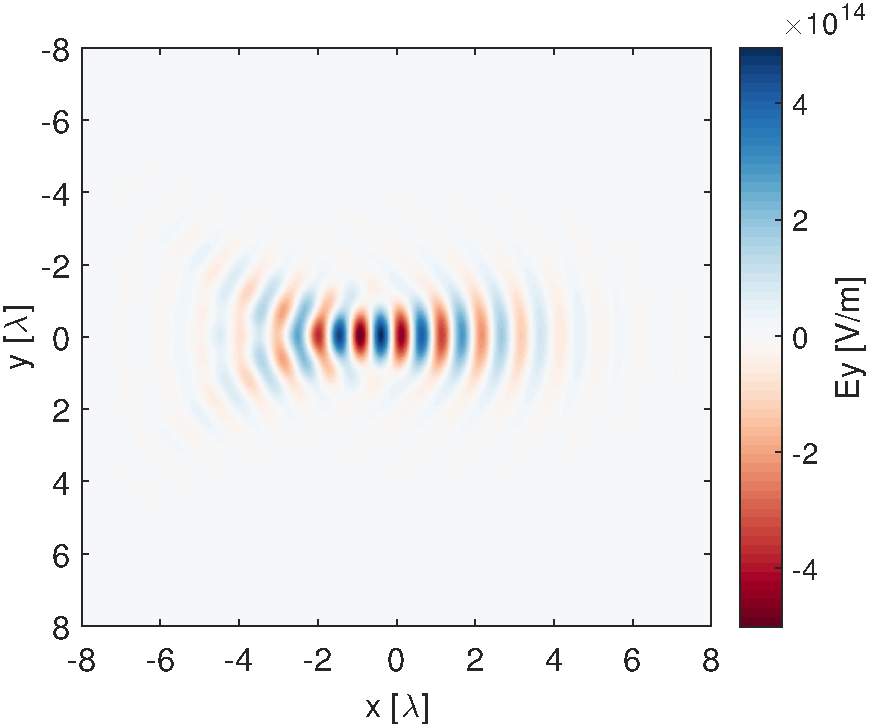
\includegraphics[width=0.44\linewidth]{./img/parax/Ey_focus.pdf}}}
	\hspace{2mm}
	\sidesubfloat[]{{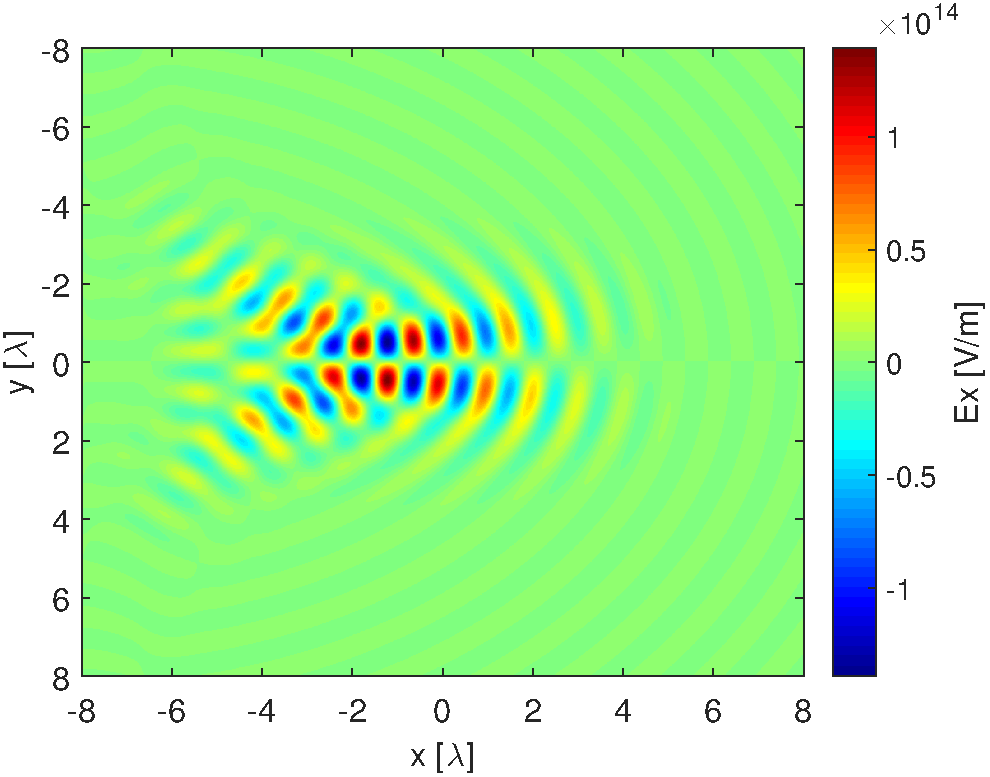
\includegraphics[width=0.44\linewidth]{./img/parax/Ex_focus.pdf}}}\\
	\sidesubfloat[]{{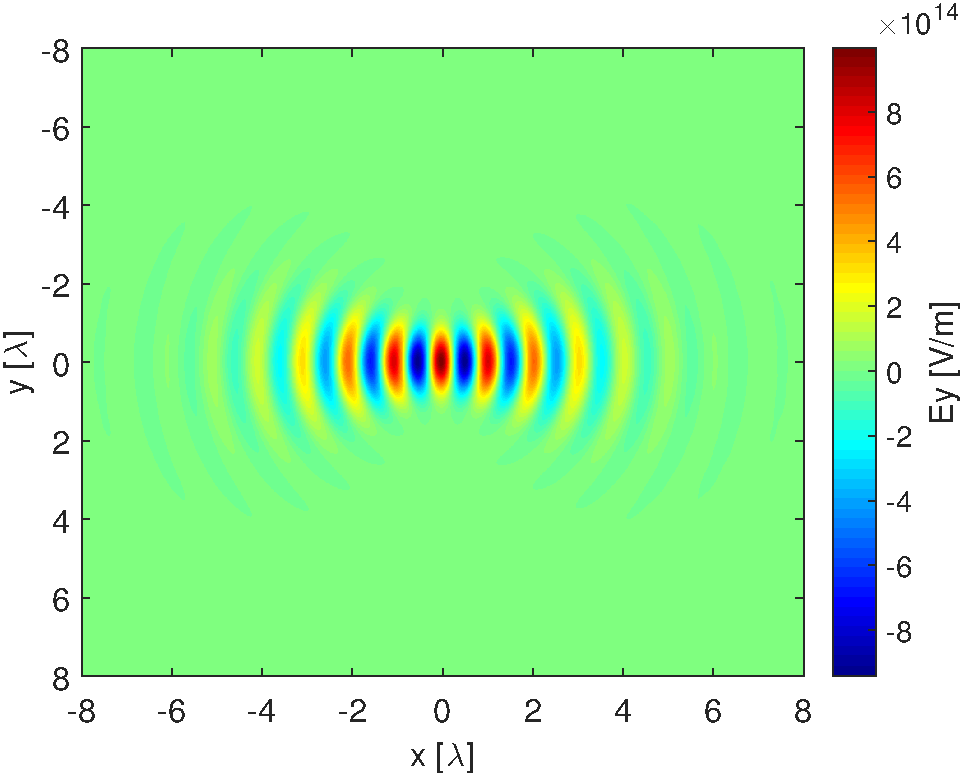
\includegraphics[width=0.44\linewidth]{./img/lbcs/Ey_focus.pdf}}}
	\hspace{2mm}
	\sidesubfloat[]{{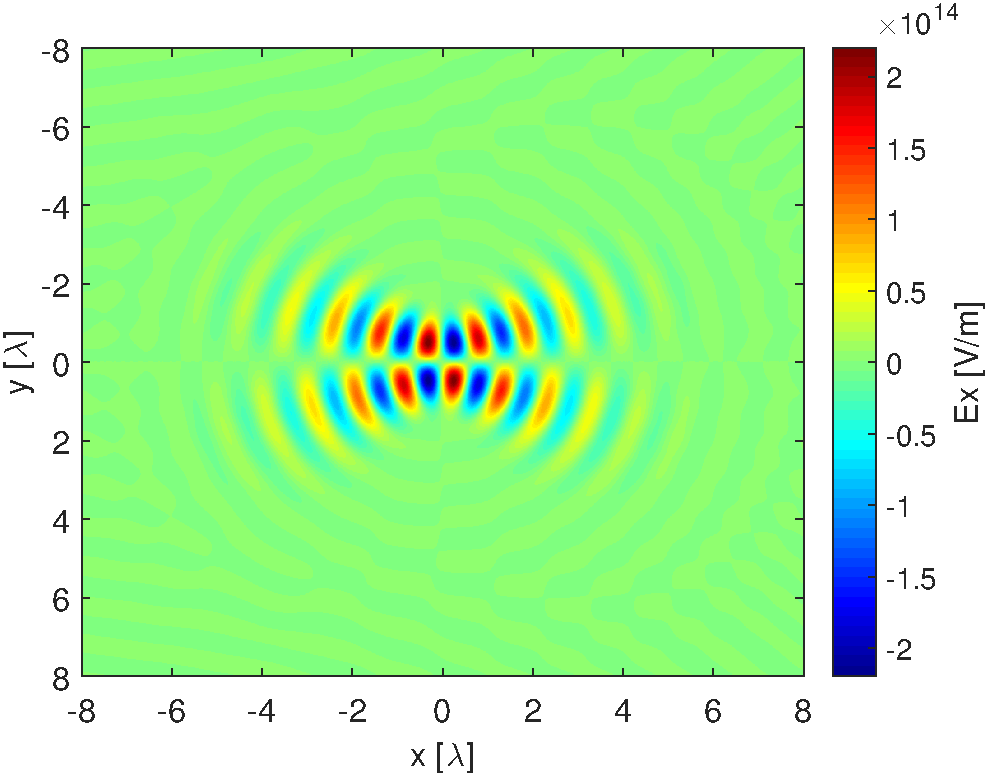
\includegraphics[width=0.44\linewidth]{./img/lbcs/Ex_focus.pdf}}}
	\caption{Transverse ($ E_{y} $) and longitudinal ($ E_{x} $) electric laser field components captured at the time step of their maximal intensity in the focal spot. The cases \textbf{(a)}, \textbf{(b)} correspond to the laser pulse propagating under the paraxial approximation, whilst \textbf{(c)}, \textbf{(d)} come from the simulation where the beam propagation has been resolved within the Maxwell consistent approach. In the case of paraxial approximation, both components reveal strong distortions and asymmetry, their focal spot is located about $ \mathrm{1 \mu m} $ closer to the left boundary than specified and the corresponding amplitude is significantly lower. The laser has been attached to the left hand side boundary.}
	\label{fig:1}
\end{figure}

Fig. \ref{fig:2} shows transverse and longitudinal slices of transverse electric field component in focus for the case of laser beam propagating under the paraxial approximation (Fig. \ref{fig:2} - a, b) as well as for the case where the beam propagation has been resolved within the Maxwell consistent approach (Fig. \ref{fig:2} - c, d). For the case of paraxial approximation, one can clearly see the asymmetry of the field shape in the longitudinal slice (Fig. \ref{fig:2} - b), which consequently leads to a decrease of the amplitude in focus and to the strong side-wings in the spatial beam profile, as might be seen from the transverse slice (Fig. \ref{fig:2} - a). On the other hand, Maxwell consistent approach calculates fields of perfect symmetry with respect to the focus (Fig. \ref{fig:2} - c) and no side-wings or distortions are present (Fig. \ref{fig:2} - d).

In Fig. \ref{fig:3} one can examine the time evolution of transverse (Fig. \ref{fig:3} - a) and longitudinal (Fig. \ref{fig:3} - b) electric field components at boundary as computed using Maxwell consistent approach. Note, that one have to chose carefully the transverse size of the domain, since the beam width at boundary may be much larger than in focus because of a diffraction.

\floatsetup[figure]{style=plain, subcapbesideposition=top}
\begin{figure}[h!]
	\centering
	\sidesubfloat[]{{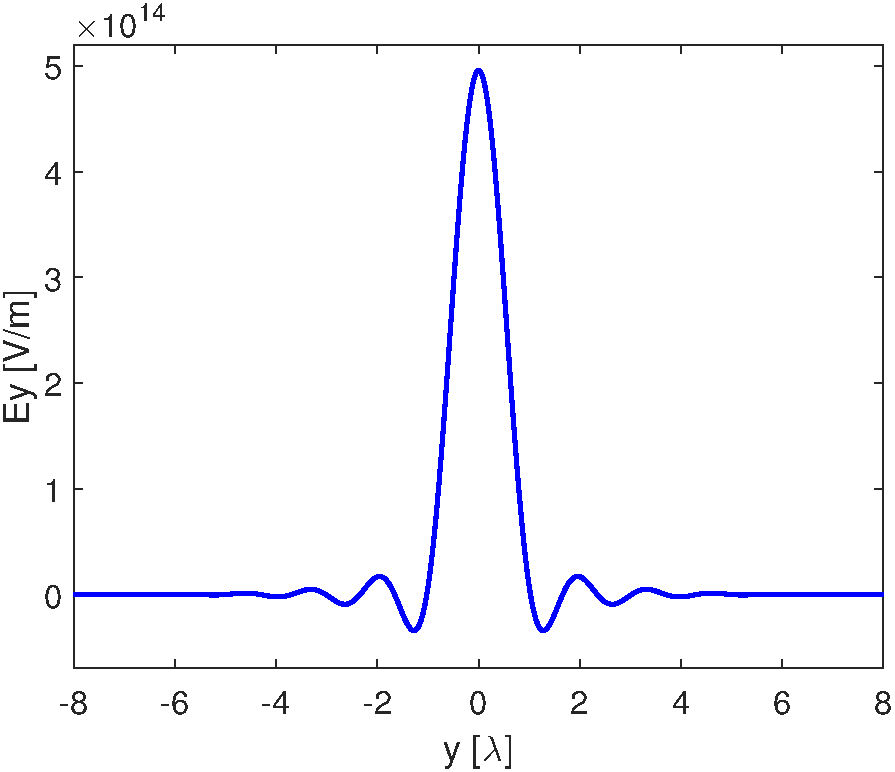
\includegraphics[width=0.4\linewidth]{./img/parax/Ey_focus_trans.pdf}}}
	\hspace{2mm}
	\sidesubfloat[]{{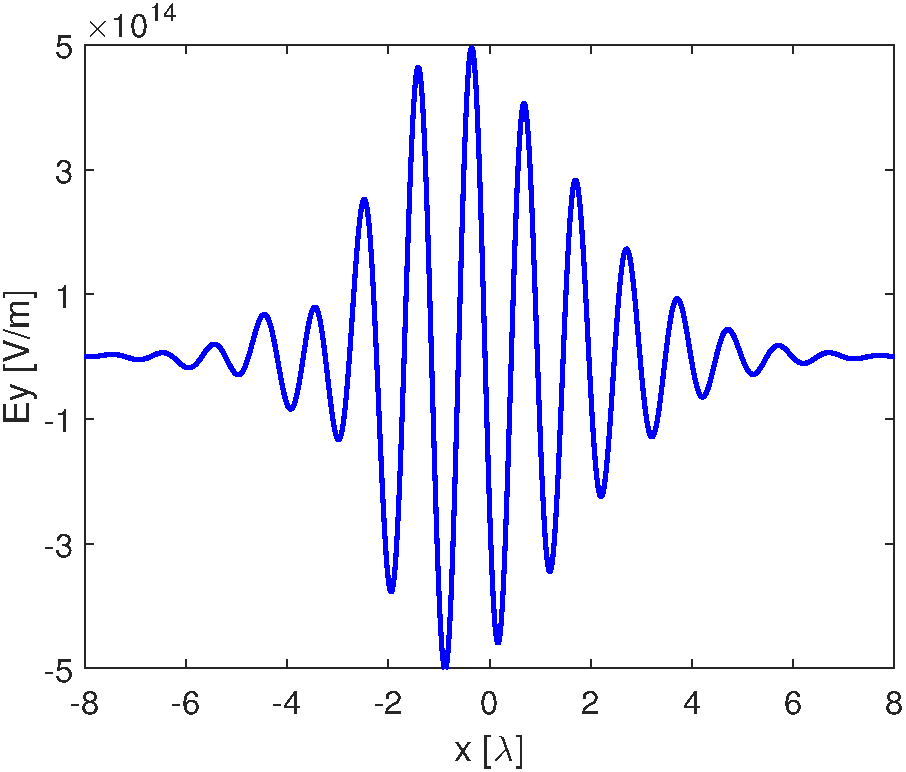
\includegraphics[width=0.4\linewidth]{./img/parax/Ey_focus_long.pdf}}}\\
	\sidesubfloat[]{{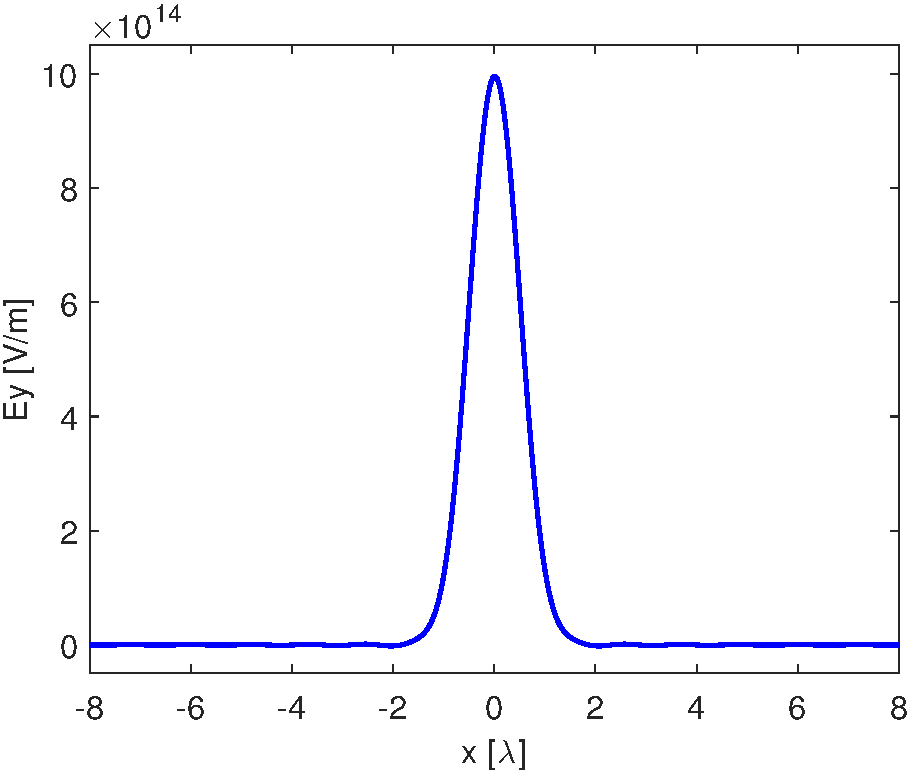
\includegraphics[width=0.4\linewidth]{./img/lbcs/Ey_focus_trans.pdf}}}
	\hspace{2mm}
	\sidesubfloat[]{{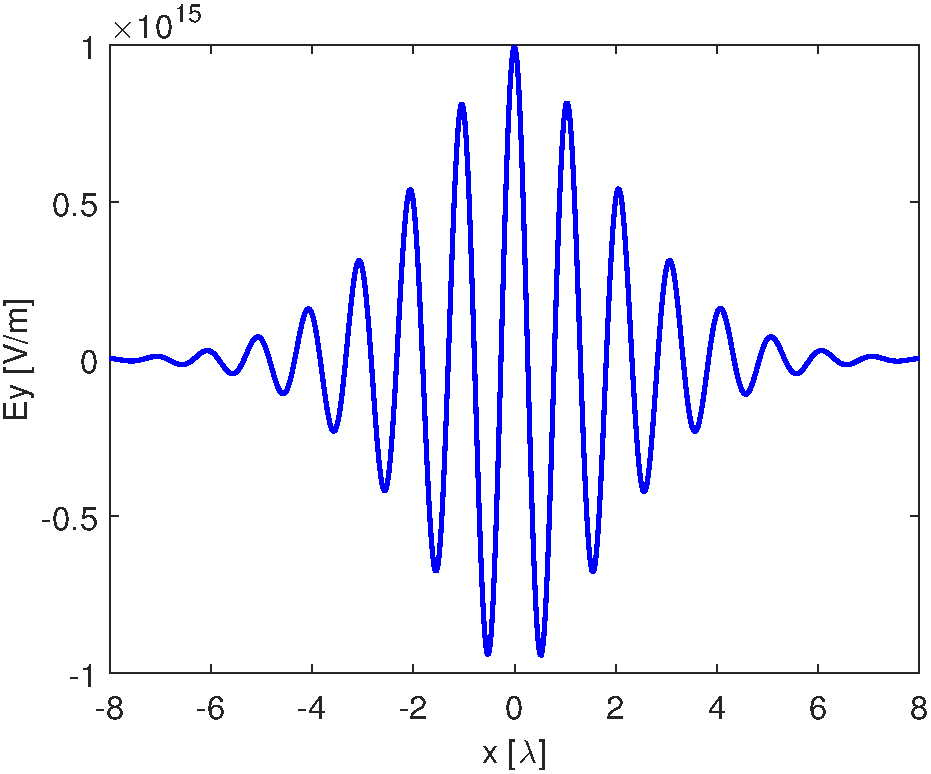
\includegraphics[width=0.4\linewidth]{./img/lbcs/Ey_focus_long.pdf}}}
	\caption{Transverse \textbf{(a)}, \textbf{(c)} and longitudinal \textbf{(b)}, \textbf{(d)} slices of the transverse electric laser field ($ E_{y} $) at the time step when it reaches maximal intensity in the focal spot. The cases \textbf{(a)}, \textbf{(b)} correspond to the laser pulse propagating under the paraxial approximation, whilst \textbf{(c)}, \textbf{(d)} come from the simulation where the beam propagation has been resolved within the Maxwell consistent approach. In the case of paraxial approximation, one can clearly see strong side-wings in the spatial beam profile \textbf{(a)} as well as the asymmetry of the field in the longitudinal line-out \textbf{(b)}.}
	\label{fig:2}
\end{figure}

To evaluate a correctness of the beam propagation using Maxwell consistent approach, several criteria has been defined. The correctness of the amplitude and beam width at focus as well as the right focus location has already been verified. Additional criteria has been set on a beam symmetry. In Fig. \ref{fig:4}, one can find a comparison of the transverse electric laser field component when it achieves its maximal intensity at front and rear boundary. One can clearly see the exact match between the field shapes at different time steps of the simulation in transverse (Fig. \ref{fig:4} - a) and longitudinal (Fig. \ref{fig:4} - b) slices. Moreover, all the aforementioned criteria has been fulfilled also in other simulations with different input parameters that are not presented here. Consequently, these observations prove the correctness of the propagation at least of the tightly focused Gaussian laser beams.

For the second simulation, all the input parameters remained the same except the beam width in focus. Now, the parameter $ w_0 = 5 \: \mathrm{\mu m} $, which is about the limit case for the beam propagating under the paraxial approximation. Thus, one would expect that the simulation results will be almost identical.

\floatsetup[figure]{style=plain, subcapbesideposition=top}
\begin{figure}[h!]
	\centering
	\sidesubfloat[]{{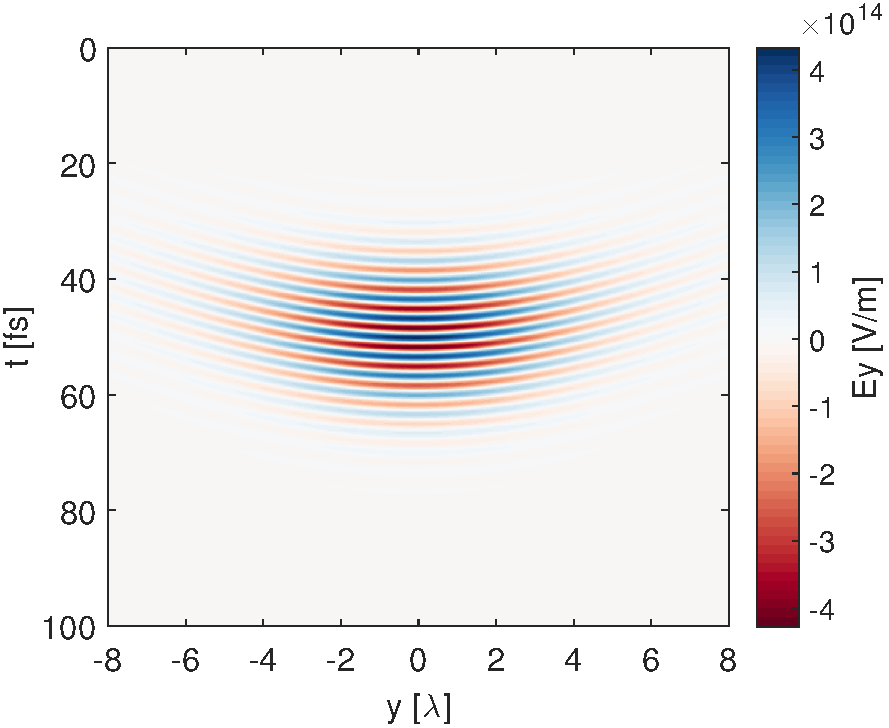
\includegraphics[width=0.44\linewidth]{./img/lbcs/Ey_boundary_time.pdf}}}
	\hspace{2mm}
	\sidesubfloat[]{{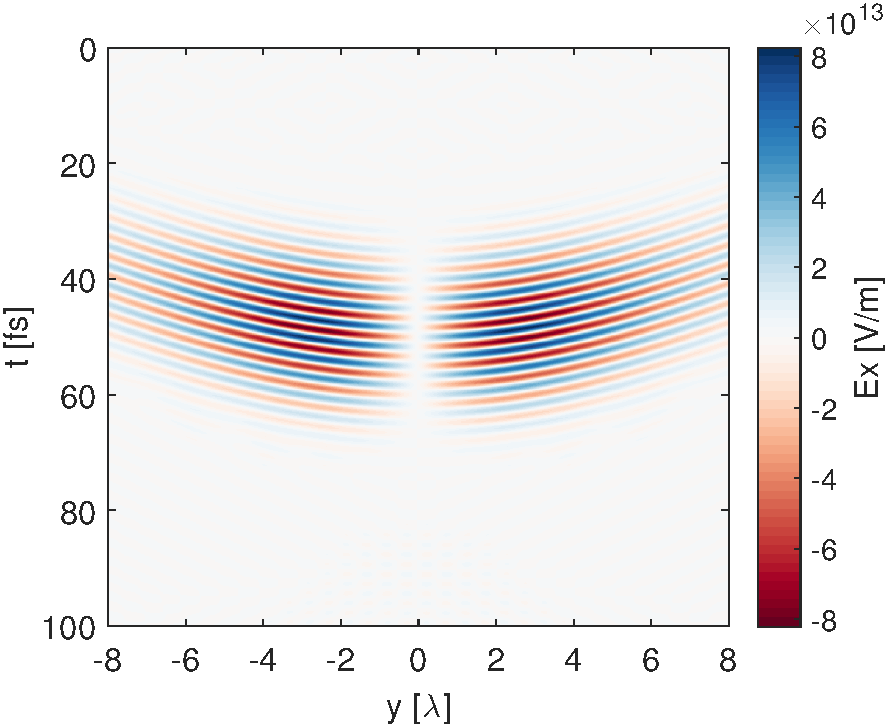
\includegraphics[width=0.44\linewidth]{./img/lbcs/Ex_boundary_time.pdf}}}
	\caption{The time evolution of transverse ($ E_{y} $) \textbf{(a)} and longitudinal ($ E_{x} $) \textbf{(b)} electric laser field components at the boundary that the laser is attached to. Both components has been calculated according to the Maxwell consistent approach.}
	\label{fig:3}
\end{figure}

\floatsetup[figure]{style=plain, subcapbesideposition=top}
\begin{figure}[h!]
	\centering
	\sidesubfloat[]{{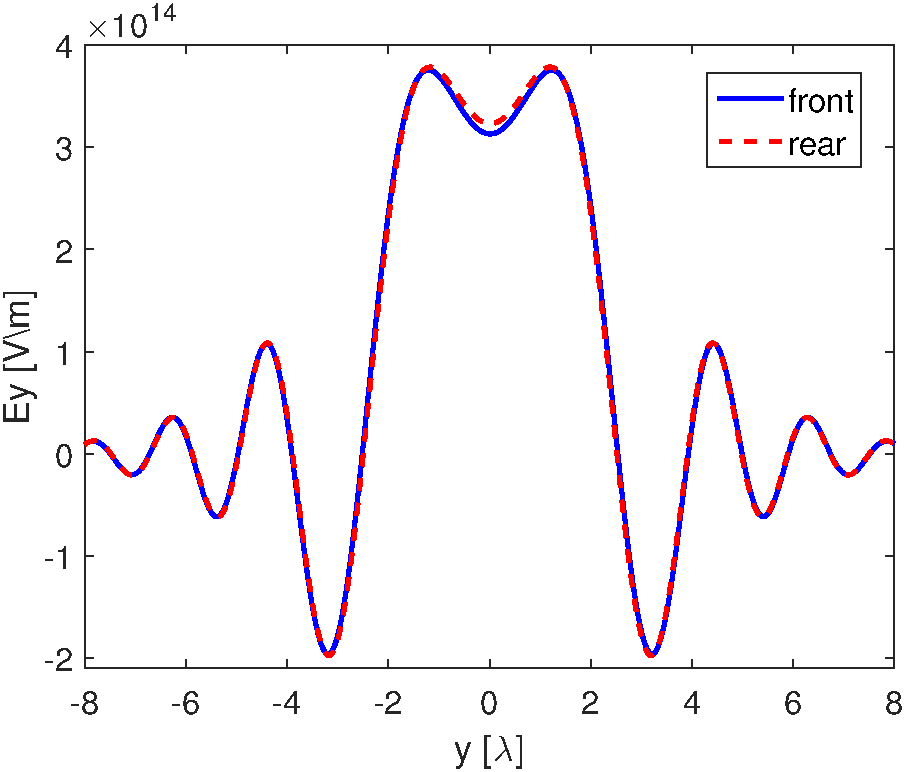
\includegraphics[width=0.44\linewidth]{./img/lbcs/Ey_boundary_trans.pdf}}}
	\hspace{1mm}
	\sidesubfloat[]{{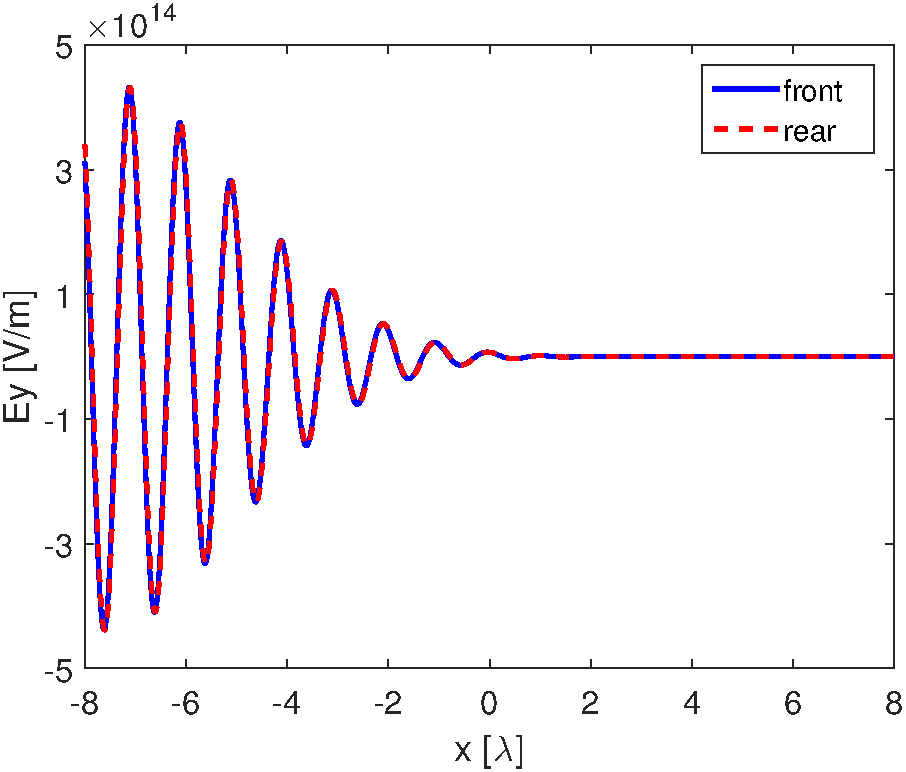
\includegraphics[width=0.44\linewidth]{./img/lbcs/Ey_boundary_long.pdf}}}
	\caption{Transverse \textbf{(a)} and longitudinal \textbf{(b)} slice of the transverse electric laser field ($ E_{y} $) when it reaches its maximal intensity at the front (blue) and rear (red) boundary. The results come from the simulation where the Maxwell consistent approach for laser propagation has been used. For better comparison, the field at the rear boundary in \textbf{(b)} has been horizontally flipped. The exact match between the field shapes at a different time steps of simulation proves the correctness of the laser beam propagation.}
	\label{fig:4}
\end{figure}

Similarly as in Fig. \ref{fig:1}, Fig. \ref{fig:5} shows again transverse and longitudinal electric field components at their maximal intensity in the focus for both cases, laser beam propagating under the paraxial approximation (Fig. \ref{fig:5} - a, b) and according to the approach consistent with Maxwell equations (Fig. \ref{fig:5} - c, d). Here, one cannot register any difference between the results corresponding to both approaches.

\floatsetup[figure]{style=plain, subcapbesideposition=top}
\begin{figure}[h!]
	\centering
	\sidesubfloat[]{{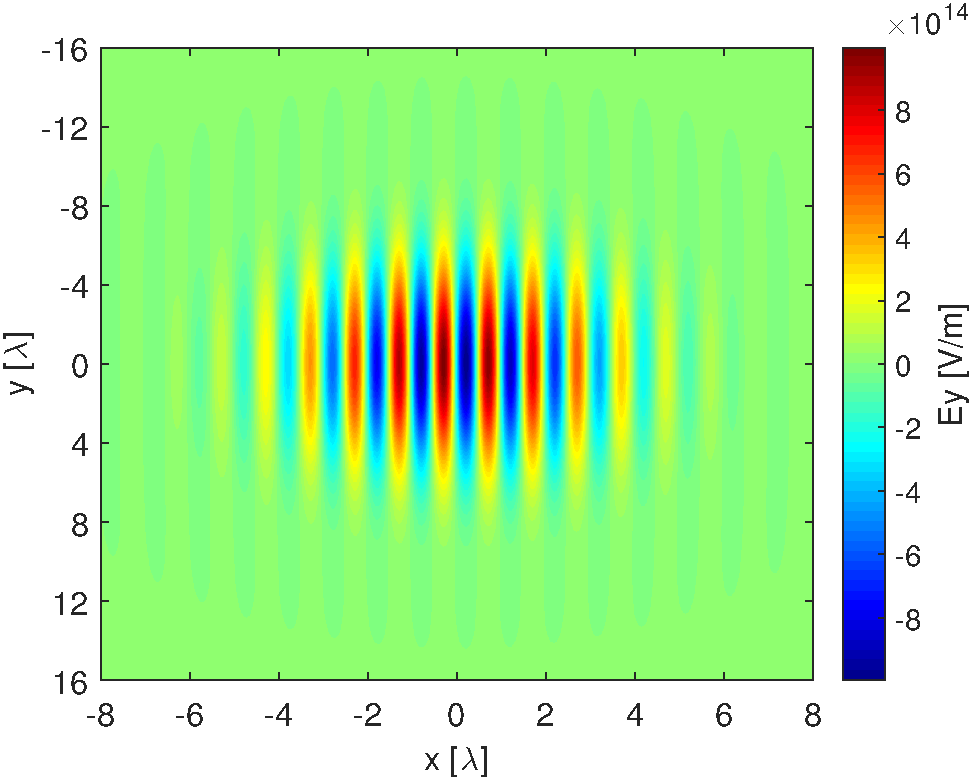
\includegraphics[width=0.45\linewidth]{./img/parax/Ey_focus_5mic.pdf}}}
	\hspace{2mm}
	\sidesubfloat[]{{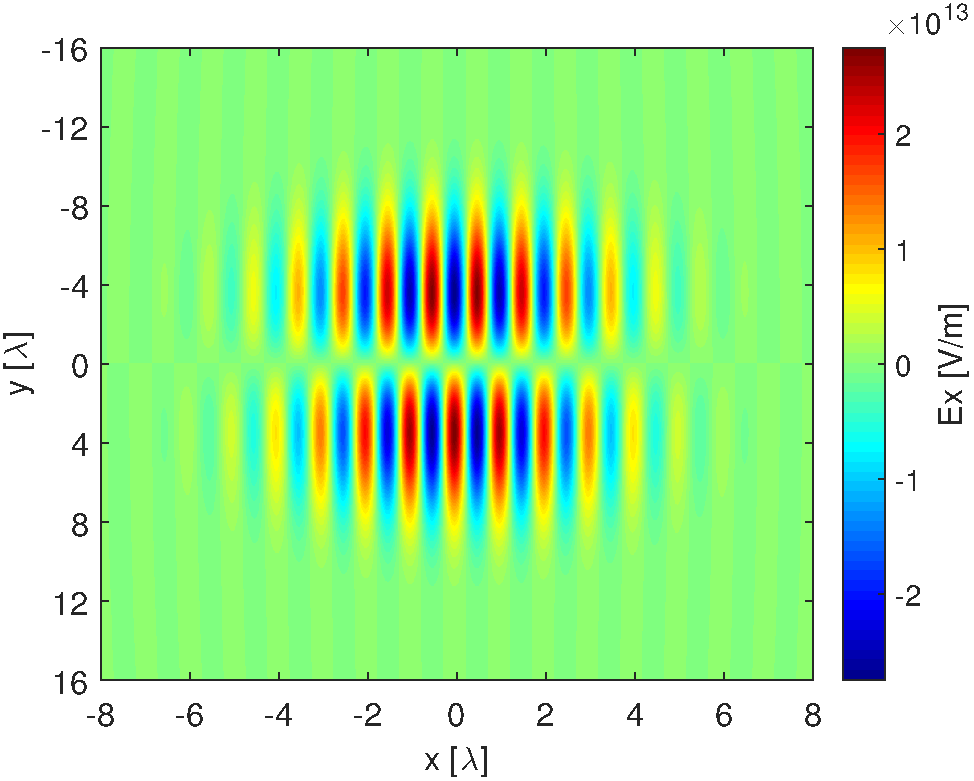
\includegraphics[width=0.44\linewidth]{./img/parax/Ex_focus_5mic.pdf}}}\\
	\sidesubfloat[]{{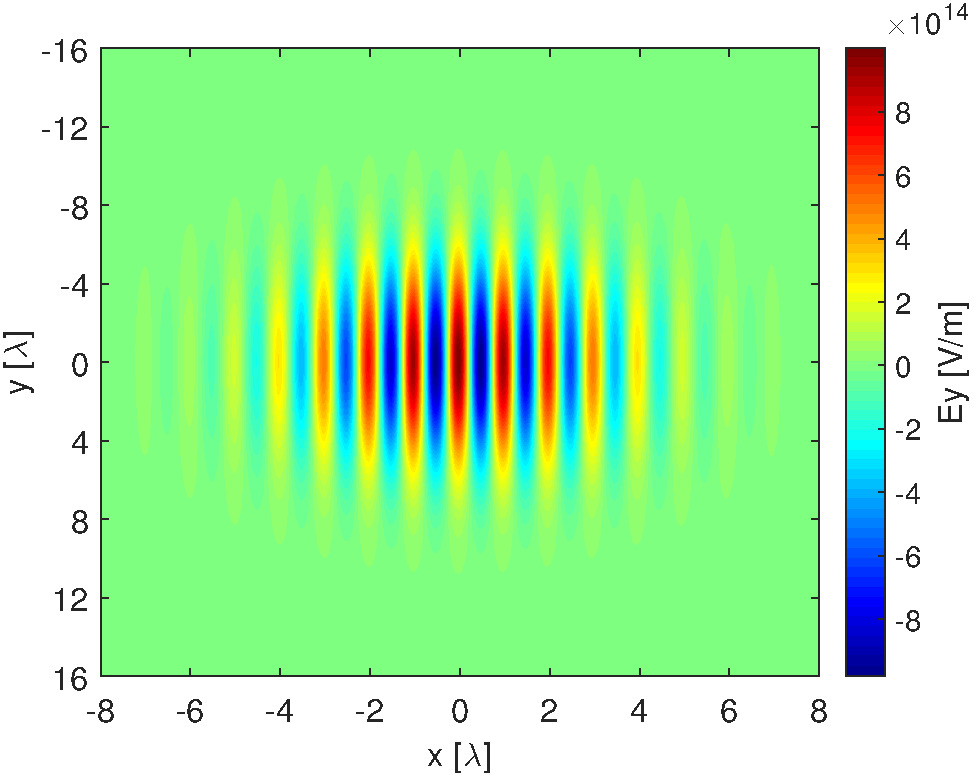
\includegraphics[width=0.44\linewidth]{./img/lbcs/Ey_focus_5mic.pdf}}}
	\hspace{2mm}
	\sidesubfloat[]{{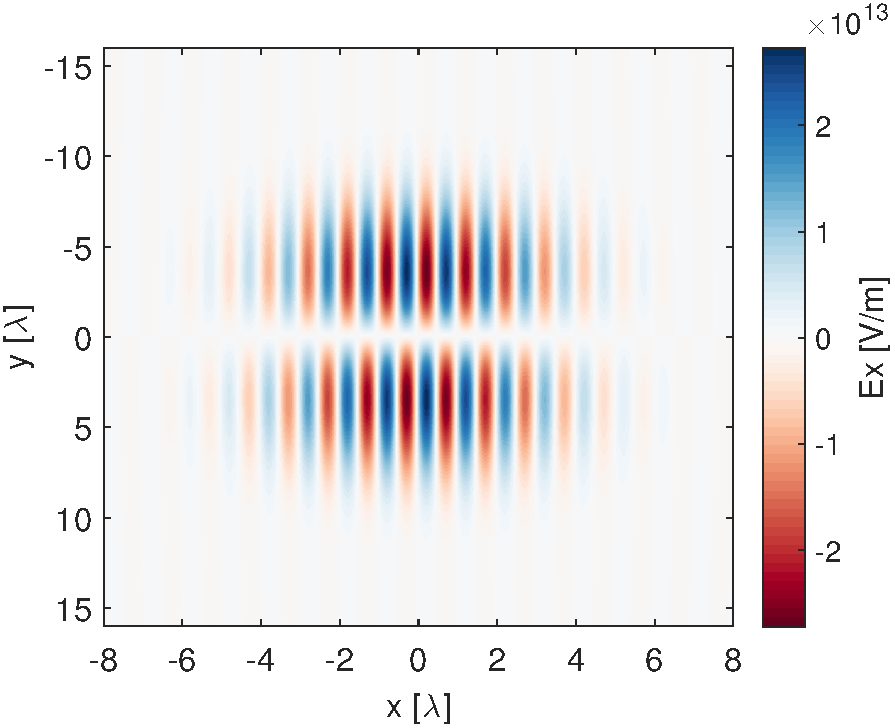
\includegraphics[width=0.43\linewidth]{./img/lbcs/Ex_focus_5mic.pdf}}}
	\caption{Transverse ($ E_{y} $) and longitudinal ($ E_{x} $) electric laser field components captured at the time step of their maximal intensity in the focal spot. The cases \textbf{(a)}, \textbf{(b)} correspond to the laser pulse propagating under the paraxial approximation, whilst \textbf{(c)}, \textbf{(d)} come from the simulation where the beam propagation has been resolved within the Maxwell consistent approach. The size of the focus has been chosen to be one order of the magnitude larger than the center laser wavelength. One can clearly see, that there is no significant difference between the shapes of the electric field components.}
	\label{fig:5}
\end{figure}

Also, the transverse slice of the transverse electric laser field component in focus (Fig. \ref{fig:6} - a) shows the correct shape and amplitude for both cases. The longitudinal slice (Fig. \ref{fig:6} - b), however, points out the fact that the location of the focus is still little bit shifted closer to the left hand side boundary. Nevertheless, this difference could be in practice neglected. At the end of the day, for the Gaussian beams propagating under the paraxial approximation, the beam diameter at focus should be at least one order of magnitude larger than the center laser wavelength.

\floatsetup[figure]{style=plain, subcapbesideposition=top}
\begin{figure}[h!]
	\centering
	\sidesubfloat[]{{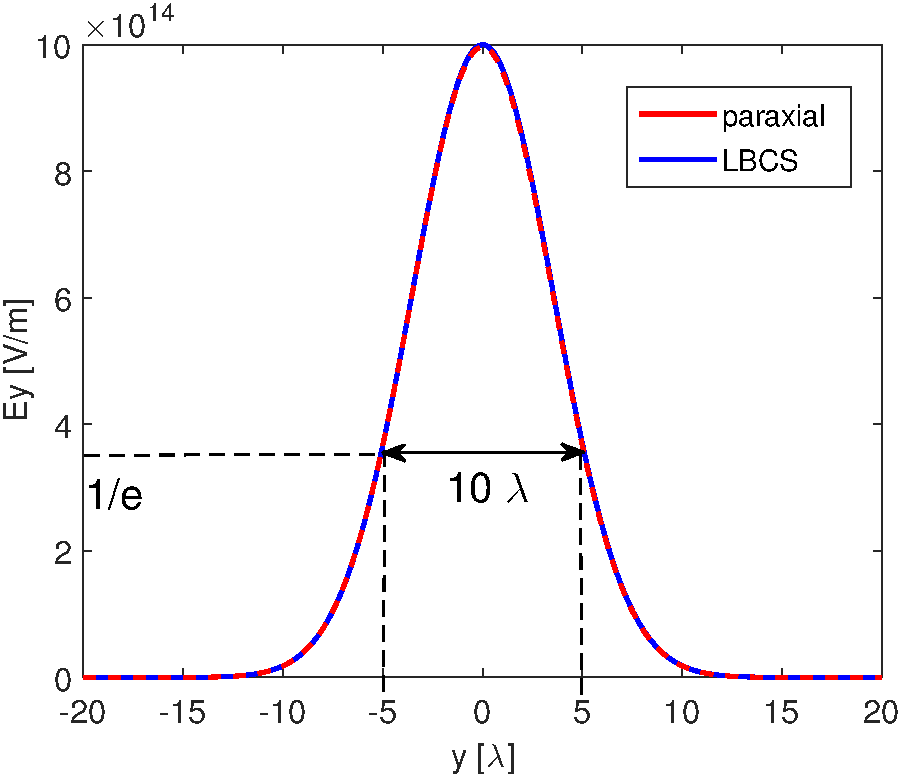
\includegraphics[width=0.44\linewidth]{./img/parax/Ey_focus_trans_comparison.pdf}}}
	\hspace{1mm}
	\sidesubfloat[]{{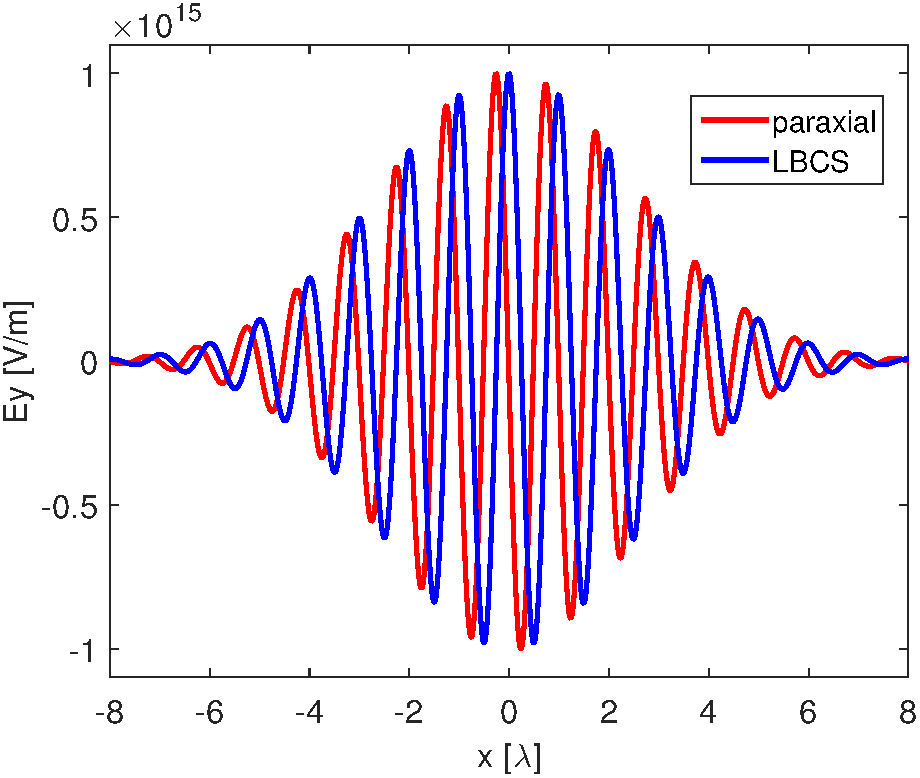
\includegraphics[width=0.45\linewidth]{./img/parax/Ey_focus_long_comparison.pdf}}}
	\caption{Transverse \textbf{(a)} and longitudinal \textbf{(b)} slices of the transverse electric laser field ($ E_{y} $) at the time step when it reaches maximal intensity in the focal spot. Red lines correspond to the laser pulse propagating under the paraxial approximation, whilst blue lines come from the simulation where the beam propagation has been resolved within the Maxwell consistent approach. The size of the focus has been chosen to be one order of magnitude larger than the center laser wavelength. In the case of paraxial approximation, the focus is slightly shifted closer to the left boundary \textbf{(b)}, otherwise the size of the focus as well as the amplitude is correct for both cases \textbf{(a)}.}
	\label{fig:6}
\end{figure}

In conclusion, one should be aware that propagation of tightly focused laser pulses cannot be described by paraxial approximation. Above, it has been shown that for the beams focused to a spot with the size comparable to a center laser wavelength, paraxial approximation leads to a shifted location of the focus, asymmetric laser field profiles with distortions and lower amplitude. These deviations are far from negligible and have without any doubt strong impact on the laser-matter interaction results. On the other hand, the propagation of tightly focused Gaussian laser beams prescribed at boundaries according to the Maxwell consistent approach has been proven to be correct.
